\documentclass{article}
\usepackage{graphicx} % Required for inserting images
\usepackage[utf8]{inputenc}
\usepackage{hyperref}
\usepackage[letterpaper, portrait, margin=1in]{geometry}
\usepackage{enumitem}
\usepackage{amsmath}
\usepackage{booktabs}
\usepackage{graphicx}
\usepackage{float}
\usepackage{hyperref}
\usepackage[flushleft]{threeparttable}
\usepackage{textcomp}
\hypersetup
{
colorlinks=true,
    linkcolor=black,
    filecolor=black,      
    urlcolor=blue,
    citecolor=black,
}




\usepackage{titlesec}
  
\title{Homework 4 Submission}
\author{David Wilson \\ Economics 7103}

  
\begin{document}
  
\maketitle

\section*{Python}

\begin{enumerate}
\item It does appear as though there is a parallel trend before the treatment.
\begin{figure}[ht]\centering
    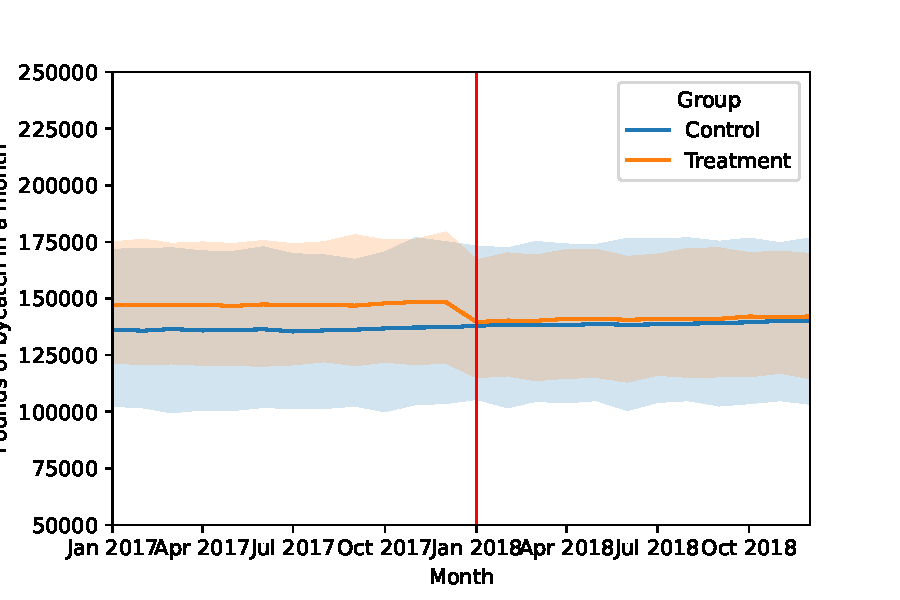
\includegraphics[width=0.7\linewidth]{trends.pdf}
    
    \caption{This graph shows the trends between treatment and control group around the policy implementation date of Jan 2018. }
\end{figure}
    
\item  Estimation of the treatment effect of the program on bycatch.

\begin{table}[H]\centering
    \begin{threeparttable}
    \caption{DID estimates}
    \label{t1:DID}
    \begin{tabular}{ll}
\toprule
 & Sample analog value \\
\midrule
$\E[Y_{igt}|g(i)=treatment,t=Pre]=$ & 148430.64 \\
$\E[Y_{igt}|g(i)=treatment,t=Post]=$ & 139612.51 \\
$\E[Y_{igt}|g(i)=control,t=Pre]=$ & 137228.60 \\
$\E[Y_{igt}|g(i)=control,t=Post]=$ & 139612.51 \\
\midrule DID= & -9591.35 \\
\bottomrule
\end{tabular}

    \begin{tablenotes}
    \end{tablenotes}
    \end{threeparttable}
\end{table}

The intuition of the DID estimate is that it measures the difference between the treatment effect of the program and the change over the same time period in the control group.

\item Estimating difference-in-difference using the following specifications:
\begin{equation}
     bycatch_{i,t} &= \alpha + \lambda_{t=2017}+ \gamma g(i) + \delta treat_{i,t} + \epsilon_{i,t} 
 \end{equation}
 \begin{equation}
     bycatch_{i,t} &= \alpha + \lambda+ \gamma g(i) + \delta treat_{i,t} + \epsilon_{i,t} 
 \end{equation}
 \begin{equation}
     bycatch_{i,t} &= \alpha + \lambda+ \gamma g(i) + \delta treat_{i,t} + \beta X_{i,t} + \epsilon_{i,t} 
 \end{equation}

The estimates for these specifications can be found below in Table 3, where equation 1 is estimated in column a, equation 2 is estimated in column b, and equation 3 is estimated in column c.

\begin{table}[H]\centering
    \begin{threeparttable}
    \caption{DID estimates}
    \label{t1:DID}
    \begin{tabular}{rccc}
\toprule
 & (a) & (b) & (c) \\
\midrule
DID estimates & -9591.35 & -8956.78 & -8436.28 \\
  & (3198.64) & (3135.04) & (2795.47) \\
\midrule Group FE & \checkmark & \checkmark & \checkmark \\
Month Indicator & \checkmark & \checkmark & \checkmark \\
Controls & $\times$ & $\times$ & \checkmark \\
Sample & Dec 2017 - Jan 2018 & Jan 2017 - Dec 2018 & Jan 2017 - Dec 2018 \\
\bottomrule
\end{tabular}

    \begin{tablenotes}
    \end{tablenotes}
    \end{threeparttable}
\end{table}
    \\
\end{enumerate} 
   
\section*{Stata}
    
\begin{enumerate}

\item Estimating DID using different specification in Stata:
\begin{table}[H]\centering
    \begin{threeparttable}
    \caption{DID estimates using two different methods in Stata}
    \label{t3:stata}
    \begin{tabular}{l*{2}{c}}
\hline\hline
                    &\multicolumn{1}{c}{(a)}&\multicolumn{1}{c}{(b)}\\
\hline
DID estimates       &    -8085.14&    -8149.06\\
                    &   (2619.21)&   (2489.02)\\
\hline
Method              &Firm indicators&Within-transformation\\
Observations        &        1200&        1200\\
\hline\hline
\end{tabular}

    \begin{tablenotes}
        \small \item Standard errors are clustered at the firm level.
    \end{tablenotes}
    \end{threeparttable}
\end{table}

    The within transformation is more accurate since it provides an estimation with lower standard deviations. It does so with the added caveat of stripping out the time-invariant variables by demeaning. 

    
   
\end{enumerate}
   

\end{document}


 2. Estimate the treatment effect of the program on bycatch using the sample analog of the population
difference-in-differences for treatment and control groups in December 2017 and January 2018. The
population difference-in-differences is:
DID ={E[Yigt|g(i) = treat, t = P ost] − E[Yigt|g(i) = treat, t = P re]} (1)
− {E[Yigt|g(i) = control, t = P ost] − E[Yigt|g(i) = control, t = P re]}. (2)
Simply report the estimate without a standard error. What is the intuition of the estimator?
3. Estimate the treatment effect using the following regression specifications and report all coefficients,
standard errors (or confidence intervals), and observations in a single table.
(a) Estimate the treatment effect of the program on bycatch using a regression-based two-period
difference-in-differences estimator with estimating equation:
bycatchi,t = α + λt=2017 + γg(i) + δtreati,t + εi,t, (3)
1
where λt=2017 is a separate intercept for the pre-period (December 2017), g(i) is an indicator that
firm i is in the treatment group, and treati,t is an indicator variable equal to one when a firm is
treated. Your estimating sample should include the observations in December 2017 and January
2018 only.
(b) Suppose you would like to use the full monthly sample to improve on what you did in the previous
question. Using the full monthly sample, estimate the treatment effect of the program on bycatch
using a regression-based difference-in-differences estimator using the regression:
bycatchi,t = α + λt + γg(i) + δtreati,t + εi,t. (4)
where λt are indicator variables for each time period. Report and interpret the results using the
same cluster-robust standard errors. How did your results change?
(c) Suppose now that you want to control for firm size and other covariates that change over time
such as pounds of shrimp and salmon harvested. Estimate the difference-in-differences regression
with added controls:
bycatchi,t = α + λt + γg(i) + δtreati,t + βXi,t + ϵi,t (5)
where Xi,t includes firm size, pounds of shrimp harvested by firm i in month t, and pounds of
salmon harvested by firm i in month t. Report and interpret the results using the same clusterrobust standard errors. How do your results change from question 1?
(d) Report the results from (a), (b), and (c) in a table with standard errors or confidence intervals
calculated using clustered standard errors at the firm level. Omit the estimates of the coefficients
on the month indicators in your table. How do these results compare to your previous calculation?